\section*{Risk reduction} \label{sec:risk}

\subsection*{Vehicle status}\label{sec:risk-vehicle}

\subsubsection*{Shock/vibration isolation}

The sensors in the flight controller’s inertial measurement unit (IMU) are vulnerable to vibrations. It introduces noise in the sensor data which can ultimately lead to crashes. In order to minimize the impact of vibrations, the Pixhawk is mounted on a gel material with vibration isolation properties.

As for shock absorption, we’re using the same landing legs as the ones on the DJI Matrice 100. Since they contain both a spring and a damping mechanism, they’re useful for absorbing shocks resulting from reasonable drops of up to about 1~m. The landing legs are fixed to the frame with 3D-printed symmetrical parts pressed against the legs and fastened with screws.

\subsubsection*{EMI/RFI solutions}

The EM noise generated by the propulsion system can be troublesome to the flight controller’s internal compass. For this reason, we use an external magnetometer mounted on the very top, as far away from the power circuitry as possible.

\subsection*{Safety} \label{subsec:risk-safety}

The main physical safety feature is a 3D-printed prop guard. It is designed to counter shocks towards the inside of the quadcopter. Identical parts are fixed under every motor using the same mounting holes. Each part offers 90-degree protection around a motor. To get an all-around, complete 360-degree protection, we added rigid carbon fiber rods between prop guards. These rods are also useful for mounting sensors.

\subsection*{Modeling and simulation} \label{subsec:risk-modelsim}

The SolidWorks software is used for the mechanical design of our custom parts. It’s also useful for the integration of all other components and to optimize usable space for sensor mounting.

\begin{figure}[h]
	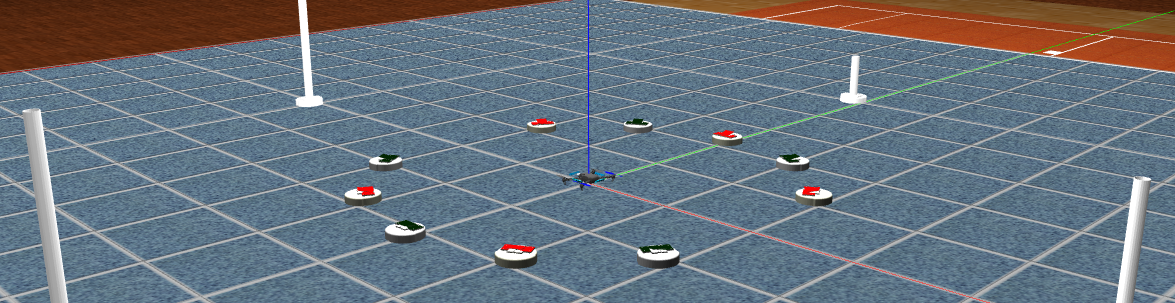
\includegraphics[width=\textwidth]{gazebo_2.png}
	\vspace{-0.5cm}
	\caption{Mission 7 simulation in Gazebo.}
	\label{fig:model-gazebo}
\end{figure}

As a part of our software development process, we use the Gazebo simulator \cite{koenig2004design} to reproduce the 7th mission’s arena and to model the physics of a quadcopter controlled by a software in the loop (SITL) version of the Pixhawk controller. We added most of the quadcopter sensors, like the 2D and 3D cameras. Our simulation also includes the floor pattern used at the competition and the 3D models of the targets and obstacles as illustrated on figure \ref{fig:model-gazebo}.

\subsection*{Testing} \label{subsec:risk-test}

\textbf{Motion capture:} Polytechnique’s Electrical Engineering Department acquired a VICON Motion Capture, allowing us to fly indoor with an external navigation system. We were then able to test all of our other modules, including target identification and pursuit, high-level strategy, and threat avoidance in an environment similar to the competition’s, without the localization module being finalized.

\textbf{Competition environment:} Last year, we acquired a 5x5 vinyl grid surface similar to the one used at the American Venue. This helped us reproduce the environment of the competition, allowing us to test our different modules more deeply than with the simulation.

\textbf{Ground and obstacle robots:} To test target detection and tracking, we have built ground and obstacle robots according to the reference instructions. However, for the control and programming of the Create 2 robots, we have decided not to use the reference Arduino setup. Instead, we mounted a Raspberry Pi 3 model B powered by a USB power bank on each robot. It runs a ROS node for the ground and obstacle robots behavior implementation and uses a driver package for serial communication \cite{roscreateautonomy}. All robots are connected via Wi-Fi to our network. Therefore, we can control and send commands to the robots with the computer used for monitoring. We can also easily remotely control the robots with a game controller.
